\documentclass[12pt,fleqn]{article}\usepackage{../../common}
\begin{document}
Materyel Mekaniği - 3

İlerlemeden önce birazdan lazım olacak iki formülü bulalım. Daha önce gördük ki

$$
I = \int \int X_2^2 \ud X_2 \ud X_3
$$

ve

$$
M = \int \int -X_2 \sigma_{11} \ud X_2 \ud X_3
$$

Üstteki iki formülü birleştirelim, $M$ içinde $I$ oluşturalım, ve yerine koyalım,

$$
M = \int \int -\frac{X_2}{X_2^2} X_2^2 \sigma_{11} \ud X_2 \ud X_3 =
-\frac{1}{X_2} \sigma_{11} I 
$$

Buradan $\sigma_{11}$ eşitliğine geçilir,

$$
\implies \sigma_{11} = -\frac{M X_2}{I}
$$

Yatay Kaykılma Stresi

Kaykılma stresi $\tau$'yu bulmak için yine çubuğun ufak bir kısmına odaklanalım,

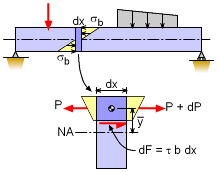
\includegraphics[width=15em]{phy_020_strs_00_06.jpg}

Tüm etki eden kuvvetlerin toplamı sıfır olmak zorundadır [2],

$$
-P + (P + \ud P) + \tau b \ud x = 0
$$

$$
-\ud P/\ud x = \tau b
\mlabel{1}
$$

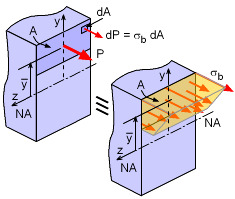
\includegraphics[width=15em]{phy_020_strs_00_07.jpg}

$P$'yi bulmak için $A$ bölgesindeki stresleri entegre ediyoruz,

$$
\int_A \ud P = \int_A \sigma_b \ud A
$$

Fakat daha önce bulduk ki $\sigma_b = -My / I$, yerine koyunca,

$$
P = \int_A - \frac{My}{I} \ud A
$$

$M$ ve $I$ sabittir, entegral dışına çıkartılabilir,

$$
P = - \frac{M}{I} \int_A y \ud A = - \frac{MQ}{I}
$$

Üstte bulunan $P$'yi (4)'e sokunca,

$$
- \frac{\ud}{\ud x} \left( - \frac{MQ}{I} \right) = \tau b
$$

$$
\frac{Q}{I} \frac{\ud M}{\ud x} = \tau b
$$

Şimdi hatırlarsak $\ud M/\ud x$ türevi yatay kaykılma yükü $V$'ye eşittir. O
zaman

$$
\frac{Q}{I} V = \tau b
$$

Nihai yatay kaykılma stres denklemi,

$$
\tau = \frac{V Q}{I b}
$$


Euler-Bernoulli çubuklarını temel alan analizleri üç adıma bölmek mümkündür.

1) Uygulanan yük $q$'yu kullanarak saptırma (deflection) fonksiyonu $y$'yi hesapla,

$$
q = E I \frac{\ud^4 y}{\ud X_1^4}
$$

Formülde görüyoruz eğer $q$ biliniyorsa ve elde yeterli sınır şartları var ise
(dört tane) diferansiyel denklemi kullanarak $y$'yi bulabiliriz
[1, Lecture 2, 2:02:00]. 

2) Saptırma $y$ bulunduktan sonra onu kullanarak kaykılma (shear) ve bükülme
momentini hesapla,

$$
M = E I \frac{\ud^2 y}{\ud X_1^2}, \quad
V = E I \frac{\ud^3 y}{\ud X_1^3} 
$$

çünkü sonuçta $M,V$ hesapları $y$'nin birer fonksiyonu, elde edilen $M,V$
sonuçları $X_1$'in fonksiyonları olacak tabii ki.

3) Oradan hareketle moment ve kaykılma $M,V$ bulunanca stres bileşenlerini
bulabilirim,

$$
\sigma_{11} = -\frac{M X_2}{I}, \quad
\sigma_{12} = -\frac{VQ}{I b}
\mlabel{2}
$$

Soru

Alttaki 6 metreli Euler-Bernoulli çubuğunun uygulanan $q$ yükü sebebiyle sahip
olacağı yer değişim fonksiyonunu bulun. Çubuğun Young genliği 20,000 MPa, ve ona
eşit şekilde dağılmış bir 45 kN / m $q$ yükü uygulanıyor. Çubuk kalınlığı 600
mm, yüksekliği 800 mm.

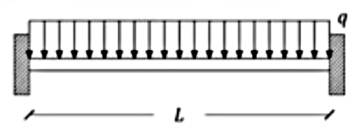
\includegraphics[width=20em]{phy_020_strs_03_02.jpg}

Çözüm

Bir dikdörtgenin atalet momenti $b h^3 / 12$. EI tabii ki Young'in genliği çarpı
bu sayı olur. Aradığımız $y$ denklemi, dördüncü dereceden bir diferansiyel
denklem çözeceğiz. Dördüncü derece demek nihai çözüm için dört tane sınır
şartı gerekli demek. Bu şartları vermeden çözersek,

\begin{minted}[fontsize=\footnotesize]{python}
import sympy as sym
L = 6000 # mm bazinda
Em = 20000
b = 500
h = 800
Ig = (b * h**3)/12
EI = Em * Ig
q = -25 # Newton icin 1000 carpip mm icin 1000 ile bolduk ayni kaldi
X1, X2 = sym.symbols('X1, X2')
y = sym.Function('y')
sol = sym.dsolve(EI*y(X1).diff(X1,4)-q, y(X1))
print (sym.latex(sol))
\end{minted}

\begin{verbatim}
y{\left(X_{1} \right)} = C_{1} + C_{2} X_{1} + C_{3} X_{1}^{2} + C_{4} X_{1}^{3} - \frac{25 X_{1}^{4}}{10240000000000008}
\end{verbatim}

`dsolve` çağrısı sıfıra eşitlik faraziyesi ile hareket ediyor, bu sebeple
üstteki çağrıda diferansiyel denklemin neye eşit olduğunu berlirtmedik.

$$
y{\left(X_{1} \right)} = C_{1} + C_{2} X_{1} + C_{3} X_{1}^{2} + C_{4} X_{1}^{3} - \frac{25 X_{1}^{4}}{10240000000000008}
$$

Çok ufak noktalı sayı [1, Lecture 2]'de 1 bolu büyük bir sayı olarak gösterilmiş,

\begin{minted}[fontsize=\footnotesize]{python}
print (1/(25./10240000000000008.))
\end{minted}

\begin{verbatim}
409600000000000.3
\end{verbatim}

$$
y{\left(X_{1} \right)} = C_{1} + C_{2} X_{1} + \frac{C_{3} X_{1}^{2}}{2} + \frac{C_{4} X_{1}^{3}}{6} - \frac{ X_{1}^{4}}{409600000000000}
$$

Gördüldüğü gibi çözümde 4 tane sabit var, bu sabitler orada çünkü sınır
şartlarını tanımlamadık. Onlar tanımlanınca sabitler yokolur.

\begin{minted}[fontsize=\footnotesize]{python}
y1 = y(X1).subs(X1,0)
y2 = y(X1).subs(X1,L)
th = y(X1).diff(X1)
th1 = th.subs(X1,0)
th2 = th.subs(X1,L)
sol = sym.dsolve(EI*y(X1).diff(X1,4)-q, y(X1),ics={y1:0,y2:0,th1:0,th2:0})
print (sym.latex(sol))
\end{minted}

\begin{verbatim}
y{\left(X_{1} \right)} = - \frac{25 X_{1}^{4}}{10240000000000008} + \frac{12500 X_{1}^{3}}{426666666666667} - \frac{37500000 X_{1}^{2}}{426666666666667}
\end{verbatim}

$$
y{\left(X_{1} \right)} = - \frac{25 X_{1}^{4}}{10240000000000008} + \frac{12500 X_{1}^{3}}{426666666666667} - \frac{37500000 X_{1}^{2}}{426666666666667}
$$

\begin{minted}[fontsize=\footnotesize]{python}
y = sol.rhs
V = EI * y.diff(X1,3)
M = EI * y.diff(X1,2)
print (V)
print (M)
\end{minted}

\begin{verbatim}
74999.9999999999 - 25.0*X1
-12.5*X1**2 + 74999.9999999999*X1 - 74999999.9999999
\end{verbatim}

Stres ogesini hesaplayabilirim simdi, formulleri (2)'de,

\begin{minted}[fontsize=\footnotesize]{python}
S11 = -M * X2 / Ig
print (sym.simplify(S11))
\end{minted}

\begin{verbatim}
X2*(5.85937499999999e-10*X1**2 - 3.515625e-6*X1 + 0.003515625)
\end{verbatim}

\begin{minted}[fontsize=\footnotesize]{python}
Q = b*((h/2) - X2) * ((h/2)+(X2/2))
S12 = (-V * Q) / (Ig*b)
print (S12)
\end{minted}

\begin{verbatim}
9.375e-14*(200000.0 - 500*X2)*(25.0*X1 - 74999.9999999999)*(X2/2 + 400.0)
\end{verbatim}


\begin{minted}[fontsize=\footnotesize]{python}
u = sym.lambdify(X1, y,'numpy')
x = np.linspace(0,L,20)
plt.plot(x,u(x))
plt.savefig('phy_020_strs_03_03.jpg',quality=30)
\end{minted}

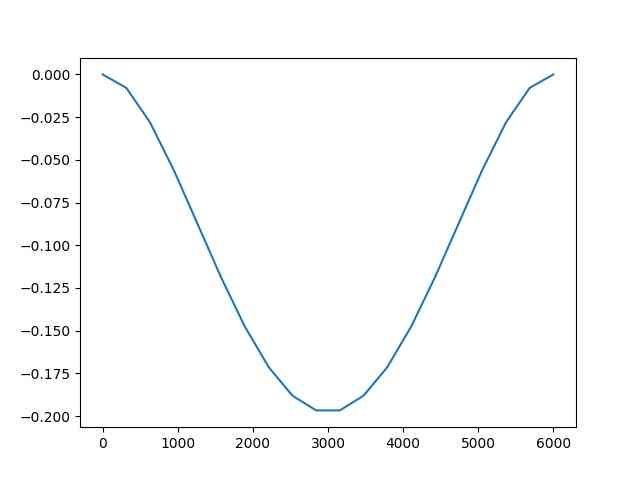
\includegraphics[width=20em]{phy_020_strs_03_03.jpg}


[devam edecek]

Kaynaklar

[1] Petitt, {\em Intro to the Finite Element Method}, University of Alberta,
    \url{https://www.youtube.com/watch?v=2iUnfPRk6Ro&list=PLLSzlda_AXa3yQEJAb5JcmsVDy9i9K_fi}

[2] Gramoll, {\em Mechanics},
    \url{http://www.ecourses.ou.edu/cgi-bin/ebook.cgi?topic=me}

\end{document}
